rsection{Timing Compartments}

This section introduces a new architecture abstraction, called timing 
compartments.
We first discuss the class of timing channels that timing compartments are 
designed
to prevent.  Then, we define the timing compartment, describe our threat model,
and discuss application scenarios that timing compartments enable.


\subsection{Taxonomy of Timing Channels}

%    \begin{figure}
%        \begin{center}
%            \includegraphics[width=2.2in]{figs/taxonomy.pdf}
%            \caption{The taxonomy of timing channels}
%            \label{fig:taxonomy}
%        \end{center}
%    \end{figure}

Timing channels are a vulnerability that occurs whenever an adversary can 
correlate the timing of an event with secret data.
They are exploited as side channels attacks that extract secret data (typically 
cryptographic keys), or covert channel attacks that bypass restrictions on 
communication.

%Figure~\ref{fig:taxonomy} summarizes the taxonomy of timing channels.  
%\emph{Direct} or language level timing channels can be identified by examining 
%the source code \cite{mitigation3}. A password checking algorithm that stops as 
%soon as an incorrect character is found causes a direct timing channel that 
%leaks information about the correct password. In contrast, \emph{indirect} or 
%microarchitectural timing channels cannot be identified in the source code 
%since they depend on hardware level behavior \cite{mitigation3}. Conventional 
%caches cause an indirect timing channel whenever the probability of a cache hit 
%depends on secret data. Programming language techniques have been developed to 
%address language level timing channels 
%\cite{timesens,mitigation1,mitigation2,mitigation3}. It is possible to reduce 
%the information leaked by some microarchitectural timing channels at the 
%language level \cite{mitigation3}. However, eliminating all leakage caused by 
%microarchitectural timing channels is difficult without hardware support.
%%%% More precise, wordier version:
%  However, efficiently providing strict timing-sensitive noninterference in the 
%  presence microarchitectural timing channels without the support of hardware 
%  is a hard problem.

Timing channels can be classified as external or internal.
\cite{mitigation3}.  In an {\em external} timing channel, the adversary measures 
the timing of a victim event and correlates it with victim data.  External 
timing channels are not caused by timing variation in the victim program rather 
than interference, and therefore can be exploited by an adversary that is 
external to the system.
%% For example, a password checking program that sequentially compares strings
%% and stops on the first incorrect character leaks the location of a mismatch.
For example, Bernstein's attack~\cite{bernstein} exploits data-dependent
timing variations in a popular implementation of AES encryption.  In the 
vulnerable program, victim cache timing events depend on the secret and affect 
the total execution time. The adversary measures the victim execution time and 
correlates this with the secret key.
Language-level techniques have been developed to
eliminate \cite{timesens} or mitigate \cite{mitigation1,mitigation2,mitigation3} 
external timing channels.

%further divided into internal or external timing channels. \emph{External} 
%timing channels are not caused by interference, and are exploited by an 
%adversary that directly measures the timing of the victim's actions. External 
%timing channels can be exploited by an adversary that does not share hardware 
%with the victim. Bernstein's attack~\cite{bernstein} exploits an external 
%timing channel in popular implementations of AES (such as OpenSSL). The 
%external timing channel exists because the cache access pattern both affects 
%the overall execution time of the AES implementation and depends on the secret 
%key. The adversary carries out the attack without sharing any hardware by 
%directly measuring the response times of the victim machine.
%%%%% The long explanation
% The adversary uses a copy of the same AES implementation as the victim to time 
% the encryption of a number inputs with a known key on the adversary's local 
% machine. Then, the adversary makes requests to the victim machine using the 
% same inputs and times how long the victim machine takes to encrypt the inputs 
% with an unknown key. In both cases, the execution time depends on the cache 
% access pattern which depends on the key. The adversary can use the timing 
% information gathered with the known and unknown keys to learn the secret AES 
% key.

Internal timing channels exist when one program's timing depends on another
program that shares the same hardware due to interference. Unlike external 
timing channels, {\em internal} timing channel vulnerabilities are caused by 
interference in shared resources.
They are exploited by an adversary that executes on hardware that it shares with 
the victim.
For example, Percival~\cite{percival} showed an internal timing channel
through a shared cache where an adversarial program can extract an AES key
by measuring its own cache access time. The victim program interferes with the 
adversary in the cache allowing the adversary to correlate its own timings with 
the key.

\subsection{Definition of Timing Compartments}

Timing compartments are a new architecture abstraction that allows software to
explicitly control {\em internal timing channels} that in shared systems.
When used in conjunction with access
control mechanisms, such as conventional page handlers, they complete software 
isolatio, because timing channels are the only side/covert channels that can be
exploited in software without physical attacks.

As a software level abstraction, a timing compartment consists of one or more 
software entities such as threads, processes, and virtual machines.  Timing 
channels between timing compartments are allowed or prevented based on a policy 
specified in software.  Policies are specified by a lattice of security levels
%where leakage is prevented from preceeding levels to preceded levels.
%of a lattice model, which defines ordering between security levels 
\cite{denning}.
This lattice model is quite expressive and widely used for information flow 
control. 
%  For example, the lattice may restrict timing channels only in one direction 
%  from $\mathtt{TC1}$ to $\mathtt{TC2}$ ($\mathtt{TC2} \leq \mathtt{TC1}$).
%  The lattice may disallow any timing channel between two compartments by 
%  making
%  them incomparable ($\mathtt{TC_1} \nleq \mathtt{TC_2}$, $\mathtt{TC_2} \nleq 
%  \mathtt{TC_1}$).

%Here, a software entitiy is some system abstraction (such as processes or 
%threads in a single OS system or virtual machines in a virtualization based 
%system) that execute software and have an owner. Intuitively, a single timing 
%compartment contains only software entities that trust each other explicitly 
%(such as all the VMs on a machine owned by the same user) or implicitly (all 
%the VMs that do not want to pay for protection), and leakage within a timing 
%compartment is safe.

Similar to other architecture abstractions such as virtual memory,
timing compartments are implemented as a combination of hardware and software
mechanisms. The underlying hardware must provide mechanisms to distinguish
events from different timing compartments and control timing interference in 
shared resources. Then, a trusted software component, which we call the timing 
compartment manager (TCM) manages the hardware mechanisms at run-time.

%To enforce the policy, a trusted software component called the timing 
%compartment manager (TCM) confines software entities into TCs. The TCM then 
%informs the hardware of the TCs and policy. At runtime, the TCM tags software 
%requests for hardware to indicate the TC of the software entity that made the 
%request. The hardware then enforces the policy by controlling how requests from 
%different TCs share resources.

Timing compartments allow software to explicitly control timing channels
among groups of software entities, but does not enforce any restrictions within
each compartment. We believe that handling timing channels separately from
traditional isolation abstractions such as processes and virtual machines is 
essential to allow efficient system designs. Because timing channel protection
is more expensive than traditional access control, a designer should be able
to pay the overhead of timing channel control only when necessary.

%Timing compartments only address timing channels; they do not control 
%information flow through explicit channels. Handling these concerns separately 
%allows for more flexibility in the overall system design.  When designing a 
%secure system, implementors must consider how the cost required to carry out a 
%particular attack compares with other attacks, the potential damage that could 
%be caused by an attack, and the cost and performance impact of implementing the 
%security mechanisms needed to stop it. This enables timing compartments to 
%provide timing channel protection only to software entities that need it.

\subsection{Threat Model}

%Goal
Timing compartments are designed to enable complete software isolation among
entities that share hardware, comparable to having separate hardware for each.
%Assumptions
Therefore, we assume that a target system has multiple cores with shared
resources such as caches, on-chip interconnects, and an off-chip memory that can
be used by multiple programs concurrently. The system can also be time shared 
(e.g. by context switching).
%The multicore system of interest consists of hardware resources that are
%concurrently shared by multiple software entities. It is possible for software 
%entities to be time multiplexed on the same core (e.g.  by context switching 
%VMs), but the system does not allow software entities to execute concurrently 
%on the same core (e.g. through simultaneous multithreading). 
We also assume that there exists a trusted software layer such as an OS or a 
hypervisor,
which provides conventional software isolation for explicit communication 
channels.
The timing compartment manager (TCM) is assumed to be a part of this trusted 
software.
In the current implementation of protection mechanisms, we also assume that
timing compartments have separate address spaces and do not share any physical
memory. Communications between timing compartments are controlled through the 
trusted
software layer and be explicitly managed to prevent external timing channels. 

%Attacks we handle.
%However, these approaches to isolate software do not address timing channels 
%that leverage shared hardware. To guarantee total isolation, internal timing 
%channels must also be eliminated. We eliminate all internal microarchitectural 
%timing channels including state and state-based timing channels.  This includes 
%all timing channels caused by concurrently shared resources as well as timing 
%channels in hardware that is shared through time multiplexing (e.g.  by context 
%switching).

Timing compartments aim to eliminate {\em internal} timing channels through
interference in shared microarchitecture resources. In particular, the goal is
to prevent both unintentional (side channel) and intentional (covert channel)
information leaks.
However, external timing
channels, which exist even without shared hardware, are not prevented by
timing compartments. If necessary, the external timing channels can be 
controlled in software. Similarly, timing channels through I/O devices are not 
considered in this study,
because they may be prevented in software.
Finally, we do not consider attacks that require physical access such as
side-channel attacks through power consumption or electromagnetic emission.

%Attacks we don't handle.
%Since our goal is to address vulnerabilities caused by hardware sharing,
%timing channels that are external to the hardware are not addressed.
%Any timing channels that are external to the hardware in this system would also 
%be present if the software entities executed on separate hardware. If 
%necessary, external timing channels can be controlled in software. Similarly, 
%we do not address language level timing channels since these may also be 
%addressed in software.  Lastly, we do not consider physical attacks and assume 
%that the adversary does not have physical access.


\subsection{Application Scenarios}

The ability to control internal timing channels can significantly increase the
level of
assurance in diverse application domains where distrusting entities share a
physical system. Here, we briefly discuss representative applications.

\subsubsection{Bring Your Own Device (BYOD)}

Now that mobile devices such as smartphones and tablets are widely used, 
companies and government organizations are starting to allow employees to
use their own devices to access the organization's data.
Bring Your Own Device (BYOD) platforms intend to enable this. However, there is 
concern that mixed use can lead to a leak of confidential data through personal 
emails or
downloaded applications. BYOD solutions such as Samsung Knox use
software containers or virtualization to separate the two environments:
personal and work. Yet, these solutions cannot prevent information leaks
through internal timing channels.

\begin{figure}
    \begin{center}
        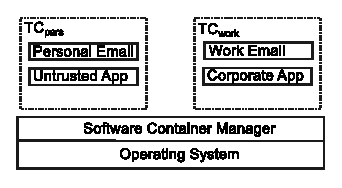
\includegraphics[width=2.79in]{figs/byod.eps}
        \caption{A BYOD example.}
        \label{fig:byod}
    \end{center}
\end{figure}

Timing compartments enable stronger isolation guarantees for BYOD
platforms. For example, consider the solution based on virtualization shown in 
Figure~\ref{app:byod}. The virtual machines for
work and personal use are assigned to two different timing compartments:
$TC_{work}$ and $TC_{pers}$. The policy is configured so that no information can 
flow from $TC_{work}$ to $TC_{pers}$.
Note that the BYOD application only requires two timing compartments even
though a system may have many cores and run many applications.

\subsubsection{High-Assurance Cloud Computing}

Infrastructure as a service cloud providers, such as Amazon EC2, lease virtual 
machines (VMs) that share physical hardware. 
%A cloud provider co-locates many VMs on a single machine to increase its 
%utilization,
%and tenants often have little control over where their VMs run.
A tenant may share hardware with competitors or attackers that want
to extract sensitive data. Conventional virtualization technologies restrict 
explicit
communication channels among virtual machines, but cannot control internal
timing channels. A practical timing channel attack has been exploited
in commercial clouds to extract cryptographic keys\cite{heyyou}.
For some clients, timing channels may not be a concern. Yet, for enterprise or 
government clients who require high assurance,
this security threat makes public cloud computing unusable. 

\begin{figure}
    \begin{center}
        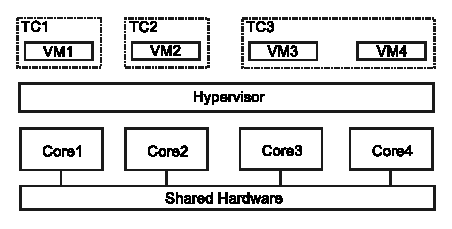
\includegraphics[width=2.79in]{figs/cloud_tcs.eps}
        \caption{A cloud computing example. VM1 and VM2 have high security 
        requirements, but VM3 and VM4 do not.}
        \label{fig:cloud_tcs}
    \end{center}
\end{figure}

Timing compartments can enable high assurance cloud computing by preventing
unintended information leakage among virtual machines.
Figure~\ref{fig:cloud_tcs} shows a cloud computing environment with four virtual 
machines (VMs).
%that have different security requirements. 
VM1 and VM2 require a strong isolation guarantee and distrust each other and 
other VMs.
VM3 and VM4 run low-security applications that do not require timing channel 
protection, but require high performance. The figure shows how three timing 
compartments can be used to meet the security requirements in this example.
VM1 and VM2 are placed in their own timing compartments $TC1$ and $TC2$, but VM3 
and VM4 are grouped in $TC3$. The policy prevents leakage out of $TC1$ and 
$TC2$, but places no constraint on timing channels out of $TC3$. This meets the 
security requirements of VM1 and VM2, but VM3 and VM4 are allowed to share 
resources normally for improved performance.


\subsubsection{Untrusted Software} 

The ability to completely eliminate timing channels enables timing compartments
to be used to contain information even when software is potentially malicious.
For example, smartphone users download third party applications
that cannot be fully trusted to manage private or sensitive data. A system may
sandbox an untrusted application and restrict its communication channels
when it accesses sensitive data. However, access control mechanisms cannot
prevent the untrusted application from leaking information to another 
unrestricted
application through internal covert timing channels. The timing compartment can 
be added to provide a complete sandbox.  In a cloud computing
context, the same timing channel protection can be used
by a cloud provider to sandbox third-party web services that cannot be fully 
trusted.

\subsubsection{Safety-Critical Systems}

In addition to protecting confidential data, the capability to control 
interference in shared hardware can also be used to provide timing guarantees on 
safety-critical systems. For example, hard real-time systems such as automotive 
controllers must meet strict timing requirements. Unfortunately, multi-core
processors cause interference that makes timing guarantees impossible. Timing
compartments can be used to ensure that the timing of safety-critical components 
are not affected by the rest of a system.

